% Agent–Environment interaction diagram – PPT colour scheme (v1 schematic)
% Compile: xelatex agent_environment_tikz_v1.tex
% Convert: pdf2svg agent_environment_tikz_v1.pdf agent_environment_tikz_v1.svg
\documentclass[border=10pt]{standalone}
\usepackage{fontspec}
\setmainfont{Aptos}[
  Path = /Applications/Microsoft Word.app/Contents/Resources/DFonts/,
  Extension = .ttf,
  UprightFont = Aptos,
  BoldFont = Aptos-Bold,
  ItalicFont = Aptos-Italic,
  BoldItalicFont = Aptos-Bold-Italic,
]
\usepackage{amsmath,amssymb}
\usepackage{tikz}
\usetikzlibrary{arrows.meta, calc, decorations.markings}

% PPT colours
\definecolor{accent}{HTML}{CB8044}
\definecolor{fg}{HTML}{E8E8E8}
\definecolor{fgdim}{HTML}{AAAAAA}
\definecolor{accentfaint}{HTML}{CB8044}

\begin{document}
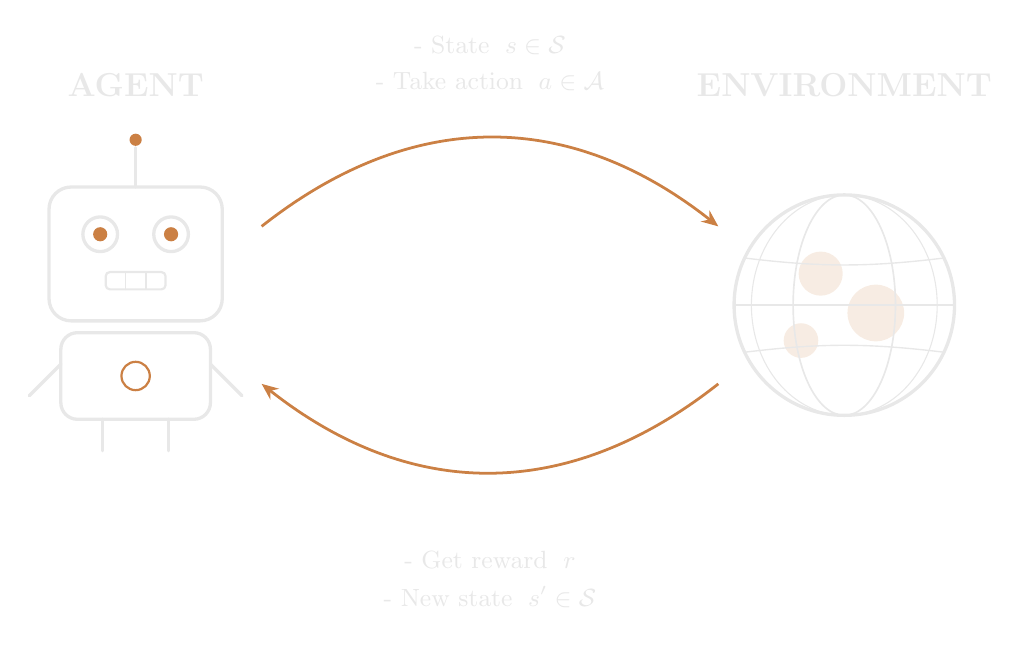
\begin{tikzpicture}[
    >=Stealth,
    curvedarrow/.style={
        accent,
        line width=1pt,
        -{Stealth[length=6pt, width=5pt]},
    },
]

% =============================================
% AGENT – Robot icon (left side, centred at 0,0)
% =============================================
\begin{scope}[shift={(0,0)}, fg, line width=1.2pt, line cap=round, line join=round]
  % Head
  \draw[rounded corners=8pt] (-1.1,0.3) rectangle (1.1,2.0);
  % Antenna stem
  \draw (0,2.0) -- (0,2.5);
  % Antenna tip
  \fill[accent] (0,2.6) circle (2.2pt);
  % Left eye
  \draw (-.45,1.4) circle (0.22);
  \fill[accent] (-.45,1.4) circle (0.09);
  % Right eye
  \draw (.45,1.4) circle (0.22);
  \fill[accent] (.45,1.4) circle (0.09);
  % Mouth
  \draw[rounded corners=1.5pt, line width=0.8pt] (-0.38,0.7) rectangle (0.38,0.92);
  \draw[line width=0.5pt] (-0.13,0.7) -- (-0.13,0.92);
  \draw[line width=0.5pt] (0.13,0.7) -- (0.13,0.92);
  % Body
  \draw[rounded corners=6pt] (-0.95,-0.95) rectangle (0.95,0.15);
  % Body accent circle
  \draw[accent, line width=0.8pt] (0,-0.4) circle (0.18);
  % Arms
  \draw (-0.95,-0.25) -- (-1.35,-0.65);
  \draw (0.95,-0.25) -- (1.35,-0.65);
  % Legs
  \draw (-0.42,-0.95) -- (-0.42,-1.35);
  \draw (0.42,-0.95) -- (0.42,-1.35);
\end{scope}

% Agent label
\node[fg, font=\fontsize{12}{14}\selectfont\bfseries] at (0,3.3) {AGENT};

% =============================================
% ENVIRONMENT – Globe icon (right side, centred at 9,0.5)
% =============================================
\begin{scope}[shift={(9,0.5)}, fg, line width=1.2pt]
  % Accent land masses (behind globe lines)
  \fill[accentfaint, opacity=0.15] (-0.3,0.4) circle (0.28);
  \fill[accentfaint, opacity=0.15] (0.4,-0.1) circle (0.36);
  \fill[accentfaint, opacity=0.15] (-0.55,-0.45) circle (0.22);
  % Main circle
  \draw (0,0) circle (1.4);
  % Vertical meridian (central)
  \draw[line width=0.6pt] (0,-1.4) arc[start angle=-90, end angle=90, x radius=0.65, y radius=1.4];
  \draw[line width=0.6pt] (0,1.4) arc[start angle=90, end angle=270, x radius=0.65, y radius=1.4];
  % Wider meridian
  \draw[line width=0.4pt] (0,-1.4) arc[start angle=-90, end angle=90, x radius=1.18, y radius=1.4];
  \draw[line width=0.4pt] (0,1.4) arc[start angle=90, end angle=270, x radius=1.18, y radius=1.4];
  % Equator
  \draw[line width=0.6pt] (-1.4,0) -- (1.4,0);
  % Latitude lines
  \draw[line width=0.5pt] (-1.28,0.6) .. controls (-0.3,0.48) and (0.3,0.48) .. (1.28,0.6);
  \draw[line width=0.5pt] (-1.28,-0.6) .. controls (-0.3,-0.48) and (0.3,-0.48) .. (1.28,-0.6);
\end{scope}

% Environment label
\node[fg, font=\fontsize{12}{14}\selectfont\bfseries] at (9,3.3) {ENVIRONMENT};

% =============================================
% TOP ARROW: Agent -> Environment
% =============================================
\draw[curvedarrow]
    (1.6,1.5) .. controls (3.5,3.0) and (5.5,3.0) .. (7.4,1.5);

% Top labels – placed above the arrow arc
\node[fg, font=\fontsize{9}{11}\selectfont, anchor=south] at (4.5,3.55) {%
  - State\; $s \in \mathcal{S}$%
};
\node[fg, font=\fontsize{9}{11}\selectfont, anchor=south] at (4.5,3.1) {%
  - Take action\; $a \in \mathcal{A}$%
};

% =============================================
% BOTTOM ARROW: Environment -> Agent
% =============================================
\draw[curvedarrow]
    (7.4,-0.5) .. controls (5.5,-2.0) and (3.5,-2.0) .. (1.6,-0.5);

% Bottom labels – placed below the arrow arc
\node[fg, font=\fontsize{9}{11}\selectfont, anchor=north] at (4.5,-2.5) {%
  - Get reward\; $r$%
};
\node[fg, font=\fontsize{9}{11}\selectfont, anchor=north] at (4.5,-2.95) {%
  - New state\; $s' \in \mathcal{S}$%
};

\end{tikzpicture}
\end{document}
